% !TEX root = paper.tex
\section{Evaluation}
\label{eval}
\name is evaluated on a commodity shared-memory machine with two 14-core
Intel Xeon CPU E5-2697 v3 processors (28 cores total) running at 2.60GHz
(turbo-boost disabled) with 756GB of memory. The operating system is
64-bit Ubuntu 16.04.5 LTS with GCC 5.5 (version 5.5.0 20171010).
\name compiler is implemented on the LLVM Compiler Infrastructure
(version 5.0.2)\cite{LLVM:CGO04}.


\name is evaluated against 12 C and C++ benchmarks, covering all the
parallelizable (exhibiting speedup) benchmarks from two
state-of-the-art automatic speculative-DOALL parallelization
papers (Privateer~\cite{johnson:12:pldi}, Cluster
Spec-DOALL~\cite{kim:12:cgo}) as well as an additional benchmark
(179.art) from HELIX~\cite{simone:12:cgo}, a non-speculative automatic
parallelization system.
We choose benchmarks that have been parallelized in prior work because this
work is focused on boosting the efficiency of automatic parallelization
rather than increasing its applicability.

% These benchmarks are from five benchmark suites (SPEC\cite{},
% PARSEC\cite{bienia:08:parsec}, PolyBench\cite{},
% MiBench\cite{guthaus:2001:iiwsc}, Trimaran\cite{trimaran:web}).
We modify the benchmarks from Polybench and \texttt{dijkstra} from
MiBench to dynamically allocate previously statically allocated arrays in order to accept
command line-defined sizes in the same way as ~\cite{johnson:12:pldi, kim:12:cgo}.
% All PolyBench benchmarks and \texttt{dijkstra} from MiBench are modified
% to accept command line arguments and allocate arrays dynamically in
% the same way as in~\cite{johnson:12:pldi, kim:12:cgo}.
%This modification is used to create bigger inputs, necessary for
%separating profiling and evaluation input sets.
%
%for exhibiting speedups on 28 cores
%
Benchmarks are profiled using small inputs, while all the
experiments presented in this section are conducted using different,
large evaluation inputs. The evaluation inputs are chosen to be large
enough for the sequential version to run for at least 10 minutes to
observe accurate parallel execution times on 28 cores. Reported speedups
are an average of 5 runs to minimize the effect of the variance in execution
time that manifests between runs.


\begin{table*}[h]
  \centering
  % !TEX root = ../paper.tex
\small
\centering
\begin{tabular}{|l|c|c|l|l|}
\hline
Benchmarks & DOALL Coverage & Sequential Time & Arguments & Input    \\
\hline
doitgen    & 99.6\%  & 1034.86 & 768 768 768 & -  \\
\hline
enc-md5    & 100.0\% & 174.26    & 1000 & -  \\
\hline
covariance & 99.9\%  &     & 4096 4096 & -  \\
\hline
swaptions  & 100.0\% & 1546.29   & -ns 10000 -sm 40000 -nt 1 & -  \\
\hline
3mm  & 100.0\%       & 3515.78   & 4096 4096 4096 4096 4096                & -  \\
\hline
gemm       & 100.0\% & 1182.50   & 4096 4096 4096                    & -  \\
\hline
179.art    & 99.1\%  & 702.32    &
{\parbox[l]{5cm}{-scanfile c756hel.in \\-trainfile1 a10.img \\-trainfile2 hc.img\\ -stride 1 -startx 60 \\-starty 90 -endx 210 \\ -endy 240 -objects 10}} & input1   \\
\hline
dijkstra-dynsize & 99.7\%  &     & ../input3000/input3000.in 3000                & input300 \\
\hline
blackscholes & 99.7\% & 4702.20   & 1 in\_10M.txt out\_10M.txt                & ref      \\
\hline
2mm  & 100.0\%       & 2360.60   & 4096 4096 4096 4096               & -  \\
\hline
052.alvinn & 97.5\%  &     & 60000                 & input 1  \\
\hline
correlation & 99.7\%  & 914.39    & 4096 4096                   & - \\
\hline
\end{tabular}
  \caption{
    Benchmark Details:
    (A) Percentage of
    execution time spent inside the parallelized loop(s). Theoretical speedup
    is calculated using Amdahl's Law with 28 workers.
    (B) Number of cross-iteration dependences
    handled by Speculation-Aware Memory Analyzer (SAMA) unresolvable by
    static analysis alone. ``N/A'' indicate all dependences are handled by static analysis.
    (C) Number of objects covered by efficient speculative
    privatization transforms proposed
    in this work.
    (D) Private read and write sizes measured using the
    evaluation input for each benchmark; v1 represents
    \name with only the planner; v2 represents \name with
    the planner and propsed enablers.}
  \label{tab:benchmark-list}
    \vspace{-5pt}
\end{table*}

\subsection{Parallelization Performance}

\begin{figure*}[ht]
  \centering
  \resizebox{0.90\textwidth}{!}{
  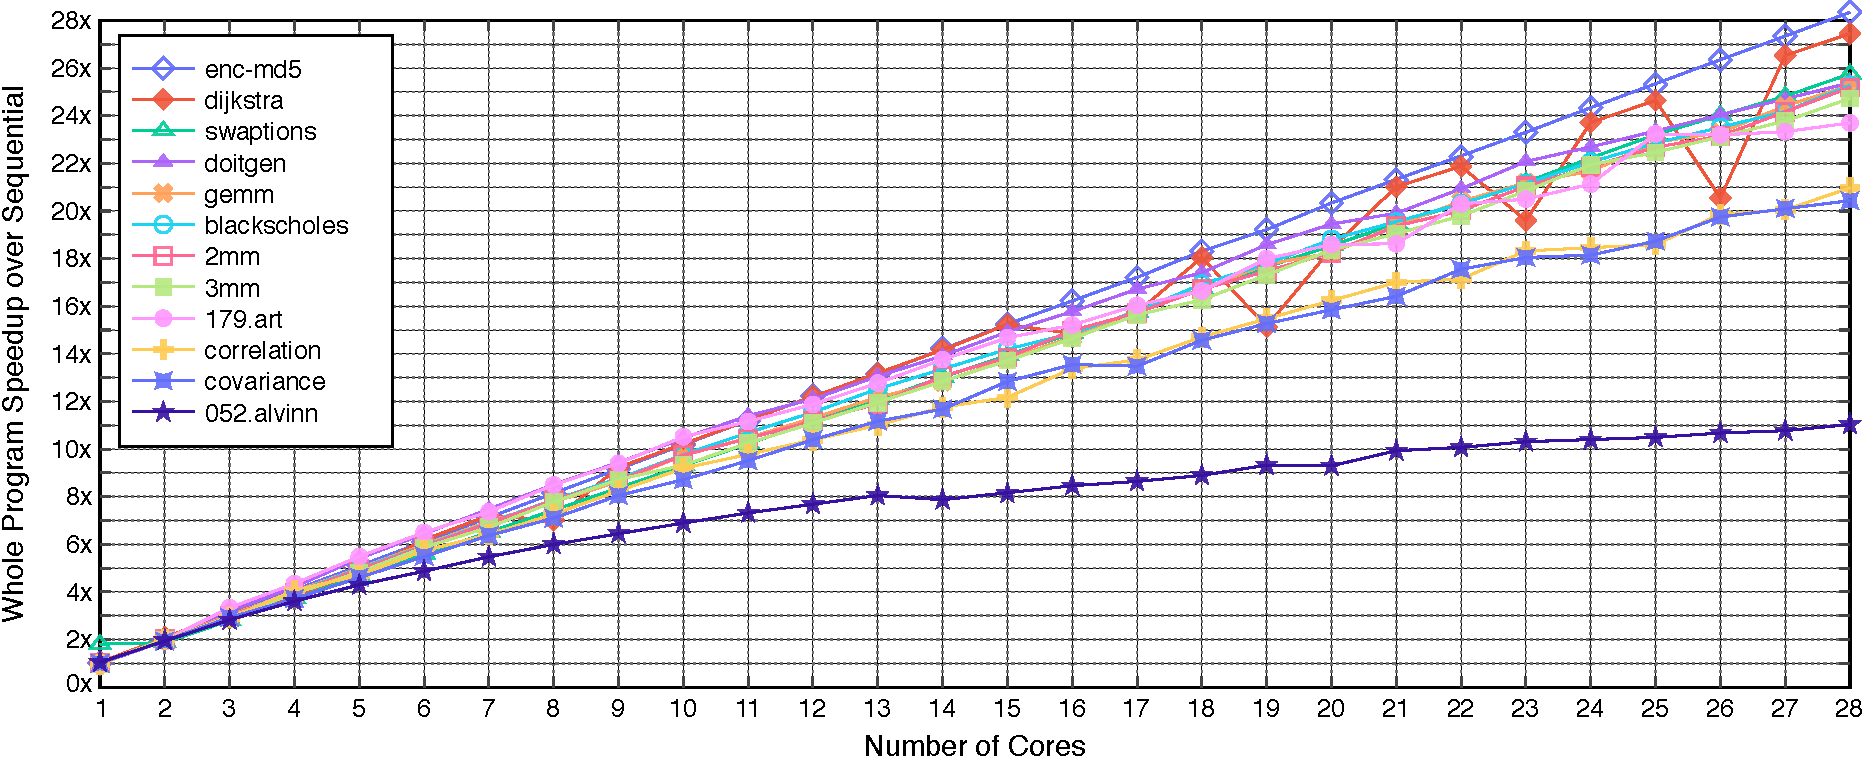
\includegraphics[width=\textwidth]{figures/multi-core-crop}
  }
  \caption{Fully Automatic Whole Program Speedup over Sequential}
  \label{fig:multi-core-scale}
\end{figure*}

Figure~\ref{fig:multi-core-scale} presents whole program speedups for
all benchmarks running up to 28 cores. These speedups are
relative to the sequential performance of the original code, compiled
with \texttt{clang++ -O3}. \name achieves scalable performance on all the
benchmarks due to the overhead reduction resulting from the use
of the speculation-aware memory analyzer and the new enablers.
To quantify their performance, Figure~\ref{fig:speedup-compare} compares
\namensp's results with Privateer and two variant of \name with various
components disabled.

% The limitations of Privateer, implemented with best practices, can be seen
% in the first bar of Figure ~\ref{fig:speedup-compare}.
We implement a version of Privateer based on the design presented in
~\cite{johnson:12:pldi} and achieve comparable speedups and runtime
overheads that scale with the larger input sets we use.
% Peephole optimizations are used to reduce the use of memory
% speculation and to hoist and combine memory checks out of the inner loop(s).
% Although we use larger inputs for evaluation, the speedups and runtime overheads
% scale with those reported in ~\cite{johnson:12:pldi}.
Despite being a
state-of-the-art framework in terms of applicability, Privateer misses
opportunities to remove read checks as mentioned in
STMLite\cite{mehrara:09:stmlite} and Cluster Spec-DOALL\cite{kim:12:cgo}.
% <<<<<<< HEAD
This is shown in (D) of Table~\ref{tab:benchmark-list}, where many
benchmarks, parallelized both speculatively and non-speculatively, have
large read sets that limit their achievable speedup. The first bar of
Figure~\ref{fig:speedup-compare} shows the manifestation of these overheads at
runtime, which are especially high for benchmarks with many reads and
writes to privatized object(s) such as \texttt{3mm}, \texttt{doitgen}, and
\texttt{dijkstra}.
% Privateer does not use static analysis and as a result has unnecessarily large read and write
% sets, especially for non-speculatively parallelized benchmarks.
% =======
% For non-speculatively parallelized benchmarks especially, Privateer does not use
% static analysis, and as a result has unnecessarily large read and write
% sets.
% >>>>>>> bbfc627307c29b03f071a18ed1a454e82d2c145f
%

Using a planner that takes into account information from static
analysis, profiling, and transforms to infer unnecessary checks on reads
of non-speculatively privatized objects reduces the read set of many
benchmarks. We notice in the second bar of Figure
~\ref{fig:speedup-compare} that \texttt{2mm}, \texttt{3mm}, \texttt{doitgen},
\texttt{enc-md5}, and \texttt{179.art} benefit from this improvement. (D)
in Table~\ref{tab:benchmark-list} reveals that for \texttt{doitgen} and \texttt{3mm},
the read set size is reduced from 2.53TB and 3TB, respectively, to zero.
The absence of these reads also allows monitoring of writes to the same
location inside the loop to be hoisted outside the loop, further decreasing
the overhead.
% To
% improve upon Privateer, we utilize static analysis
% including a stronger KillFlow analysis pass to remove read checks.
% \texttt{2mm}, \texttt{3mm}, \texttt{doitgen}, \texttt{enc-md5}, and
% \texttt{179.art} benefit from this improvement as shown in the second bar.
% Note that \textbf{ref XXX} if all dependences are removed statically, no
% checkpoint is needed in the runtime.
%

% <<<<<<< HEAD
The enablers proposed in
\cref{sec:new_enablers} takes into account specific properties of memory
objects and are able to avoid expensive monitoring of writes.
\texttt{2mm} and \texttt{3mm} have arrays that can be handled by
the independent privatization transform, avoiding monitoring any
writes and increasing the speedup, shown in the third bar of Figure
~\ref{fig:speedup-compare}, by 2$\times$ and 4.7$\times$,
respectively. In \texttt{blackscholes}, the \texttt{\textbf{prices}} array
is fully overwritten at every iteration and can be handled with the
overwrite private transform. In \texttt{dijkstra},
% =======
% The third bar shows how the addition of the enablers proposed in section
% \ref{novel_transf} to the planner affects performance. These enablers
% avoid adding expensive monitoring of writes taking into account specific
% properties of memory objects. \texttt{2mm} and \texttt{3mm} have loops in
% which each iteration writes to a different location in a privatized array.
% Since this is determined statically, we can refrain from monitoring any of
% these writes. In \texttt{blackscholes}, the \texttt{\textbf{prices}} array
% is fully overwritten at every iteration; therefore, we only need to take
% the last iteration's writes as the live-out. In \texttt{dijkstra},
% >>>>>>> bbfc627307c29b03f071a18ed1a454e82d2c145f
the \texttt{\textbf{pathcost}} array is killed at the beginning of each
iteration and similar to \texttt{blackscholes}, only requires the last
iteration's writes to be known.

Adding the speculation-aware
memory analyzer to the list of features facilitates the removal of
dependences unresolvable by static analysis.
The effect that this has is seen most prominently with \texttt{dijkstra},
where the read check of \texttt{\textbf{dist}} can be removed. The use of
control speculation in conjunction with kill-flow analysis can remove the
RAW dependence between lines \textbf{14} and \textbf{38}. Since all the
accesses to \texttt{\textbf{dist}} are contained within the loop, the local
private transform can privatize this object without any monitoring, giving
a 27.4$\times$ speedup, 4.9$\times$ over Privateer.
Dependences from \texttt{enc-md5}, \texttt{179.art}, and
\texttt{blackscholes} are also removed with this addition but they either
are rarely exhibited or are in the outer loop and do not contribute much to
the runtime overhead.
% XXX Should we talk about why or is this explained earlier in the paper?
% The remaining 3.61KB of monitored writes results from a cross-iteration
% register dependence of the induction variable, which is logged every
% iteration before a checkpoint.

\texttt{covariance} and \texttt{correlation} have complex WAW dependences
that cannot be resolved even with speculation-aware memory analyzer and
the write sets need to be monitored, limiting the achievable speedup to
20.5$\times$ and 21$\times$, respectively.

% \texttt{179.art}


% <<<<<<< HEAD
% The use of speculation-aware memory analyzer addresses dependences not
% covered by static analysis in
% \texttt{enc-md5}, \texttt{179.art}, \texttt{blackscholes}, and
% \texttt{dijkstra}, shown in (B) of Table ~\ref{tab:benchmark-list}. However,
% many of these dependences are in the outer loops (with the exception
% being \texttt{dijkstra}) and do not affect the overall performance much.
% Nevertheless, this approach is worth exploring further in future work.
% =======
% Using the speculation-aware memory analyzer addresses dependences not
% covered by static analysis in
% \texttt{enc-md5}, \texttt{179.art}, \texttt{blackscholes}, and
% \texttt{dijkstra}, shown in (B) of Table~\ref{tab:benchmark-list}. However,
% many of these dependences are in the outer loops (with the exception
% being \texttt{dijkstra}) and do not affect the overall performance much.
% Nevertheless, this approach is worth exploring further in future work.
% >>>>>>> bbfc627307c29b03f071a18ed1a454e82d2c145f
% XXX Better wording for this.

% The third bar presents the results of \name without the cheap
% privatization transformations proposed in \ref{}. Parallelization through
% \name, which incorporates speculation-aware-memory-analysis and cheap
% privatization transformations, is presented in the fourth bar, achieving
% 23.0$\times$ speedup compared to 11.5$\times$ by the original Privateer.

% enc-md5, swaptions, gemm, 3mm, 2mm, blackscholes, doitgen
% We observe close to linear scalability for \texttt{enc-md5}, \texttt{swaptions},
% \texttt{gemm}, \texttt{2mm}, \texttt{3mm}, \texttt{blackscholes},
% and \texttt{doitgen}. This performance comes from most memory
% objects being privatized with little or no overheads.

% dijkstra
% \texttt{dijkstra}, having many calls to \texttt{\textbf{malloc()}}
% inside the inner loops, shows a significant variance in
% the runtime.

% 052.alvinn
% \texttt{052.alvinn} exhibits a lower speedup (11$\times$ on 28
% cores) than other the benchmarks, resulting from the inner loop
% being chosen for parallelization. With this loop constituting 97.5\% of the
% execution time of the whole program, the theoretical max speedup is 16.7$\times$
% based on Almdahl's Law.

% 179.art
% \texttt{179.art}, whose theoretical maximum speedup is 22.5$\times$, due to
% the same effect. Note that HELIX\cite{simone:12:cgo} reports 4.2$\times$ speedup
% on 6 cores while \name exhibits 6.5$\times$, demonstrating that an efficient
% speculative approach can outperform even a static approach.

% correlation and covariance
% \texttt{correlation} and \texttt{covariance} have WAW
% dependence patterns which cannot be resolved by static analysis or cheap
% privatization variants. As a result, the corresponding memory objects are
% classified as private and need logging and merging for write sets,
% resulting in lower speedups.

\begin{figure*}[ht]
  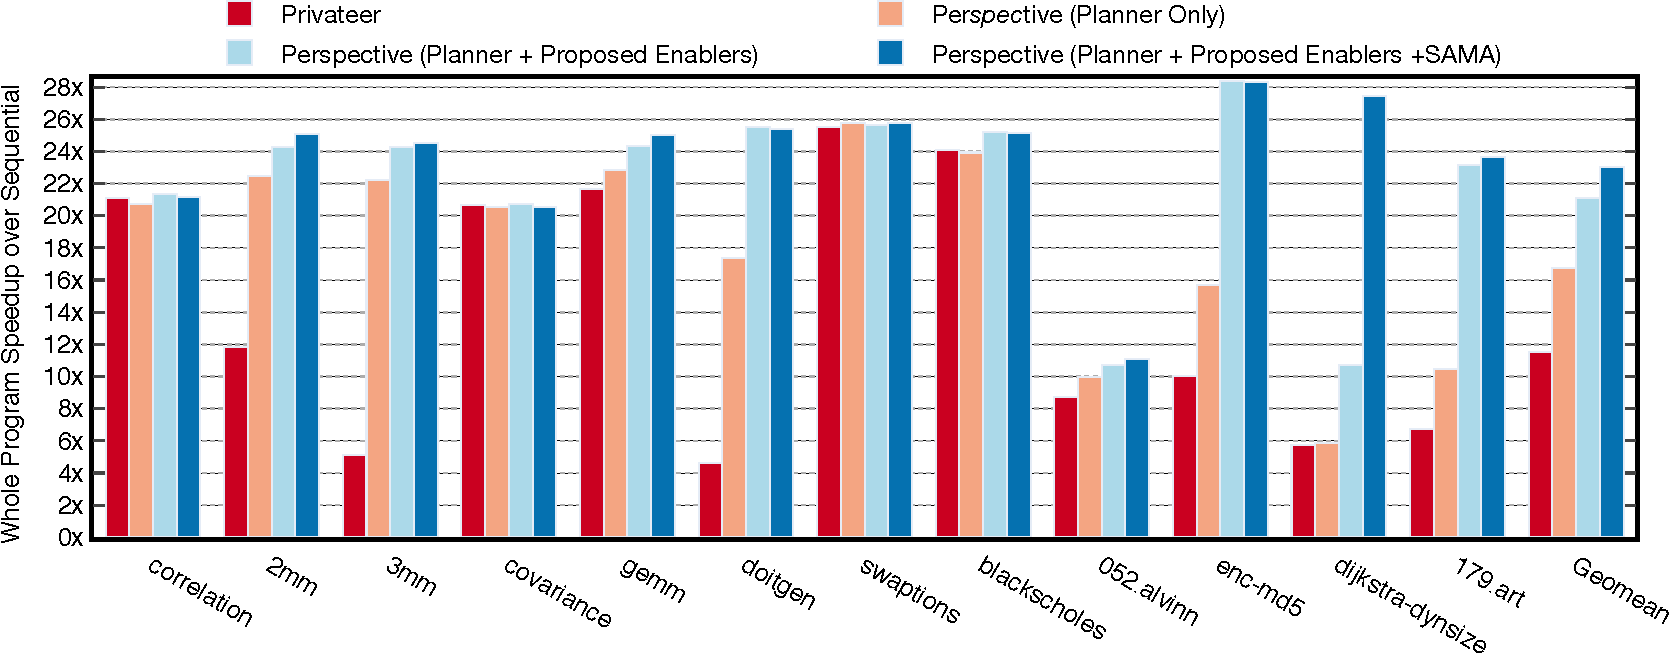
\includegraphics[width=\textwidth]{figures/compare-privateer}
  \caption{Whole Program Speedup Comparison among variants of \name and Privateer with 28 Cores}
  \label{fig:speedup-compare}
\end{figure*}



% \subsubsection{Effect of parallelization on vectorization}

% instrumentation kills vectorization


% \subsection{Static Analysis and Enablers}
% Figures Needed:
% \begin{itemize}
% % (no need, just discuss the use of CAF in previous sections) \item CAF:
% % with and without; no topping; with only BasicLoopAA and ScevAA

% % (no need, show in the benchmark table) \item Coverage: Spec-DOALL
% % percentage of coverage of each benchmark
% \item Enablers: Enablers used for each benchmark
% \item Optimization level: Performance with different optimization levels
% \end{itemize}

% Discussion Needed:

% Present in a table, which enablers were used for all benchmarks

% \subsection{Sub- and Super-Linear Speedups}
% XXX Better wording of this

% \begin{figure*}[htp]
%   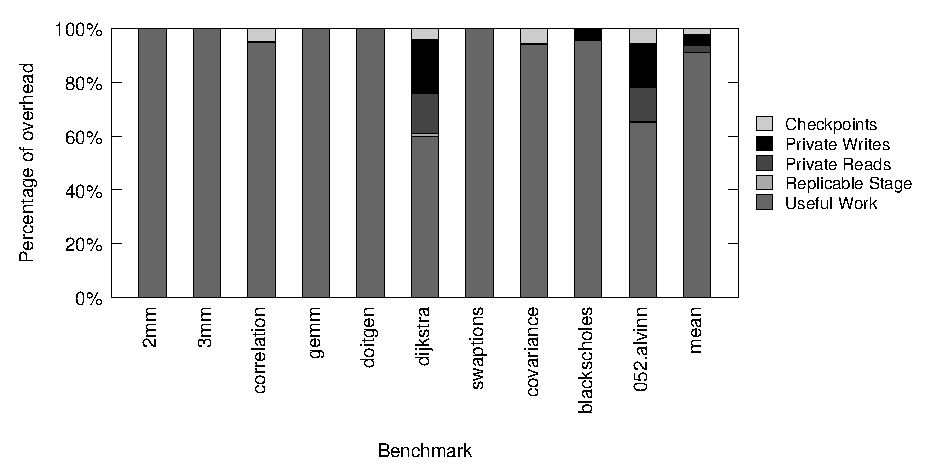
\includegraphics[width=0.9\textwidth]{figures/overheads}
%   \label{fig:overheads}
%   \caption{Overhead comparison with various enablers disabled}
% \end{figure*}
% \begin{figure*}[htp]
%   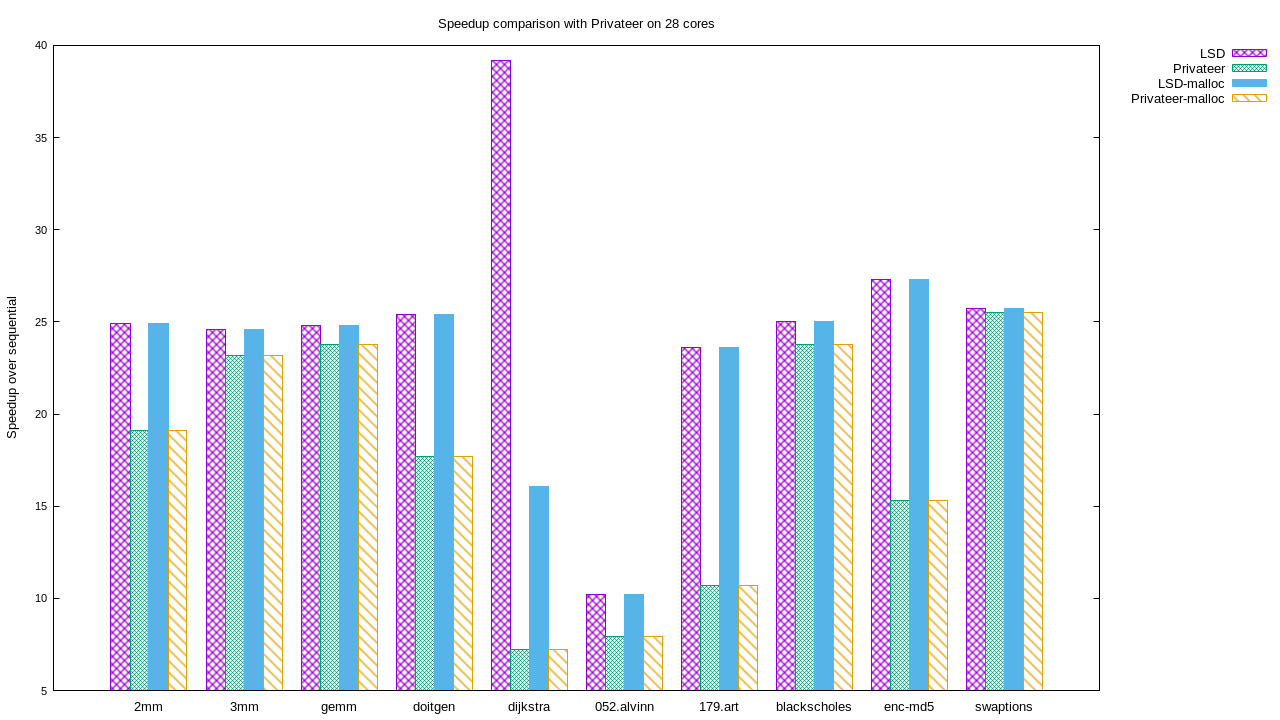
\includegraphics[width=0.9\textwidth]{figures/comparison}
% \end{figure*}
% Huge speedup for dijkstra is largely due to the cheaper "malloc" that
% we use in our heaps. Using a similar malloc in the sequential version
% yields ~16x speedup in dijkstra and insignificant difference in the
% other benchmarks.
% Shown in Figure \ref{fig:overheads} is the overhead breakdown of each
% benchmark comparing \name with various enablers disabled. The useful work
% of \name is normalized to 100\%, with the others being scaled accordingly.
% These result demonstrate the correlation between the sum of the overheads
% to the speedup that can be achieved. \{\textbf{XXX} Something about
% how we remove dependences with redundant private read elimination,
% the new kill\_private heap, and collaboration \}

% Along with adding its own overheads, the instrumentation inserted to monitor
% reads and writes can also disable other optimizations, such as
% vectorization. The use of vectorization in \texttt{052.alvinn} yields 30\%
% speedup in the sequential execution. With logging of arbitrary addresses, the loop
% vectorizer of LLVM cannot infer that these do not alias with any other
% pointer of a previously vectorizable instruction.
% XXX Is this worded horribly? Too wired to tell now

For most of the benchmarks parallelized with \namensp, checkpointing does not add any
significant (>1\%) overhead; the exceptions are
\texttt{052.alvinn}, \texttt{correlation}, and \texttt{covariance}, which
exhibit lower-than-expected speedups. % XXX ???
The inner loop of \texttt{052.alvinn} is chosen for parallelization --
because the useful work of the loop is small and runs for 60,000
iterations, checkpointing constitutes a considerable portion of the run
time, \textasciitilde20\%. For \texttt{covariance} and \texttt{correlation},
the use of the basic privatization transform entails the checkpoints merge large private sets
with an overhead of \textasciitilde10\% for each.

For several benchmarks, we observed speedups that exceed their theoretical
limits, which we attribute to two factors:
(1) We replace all calls to \texttt{\textbf{malloc()}} inside a parallelized
loop with our own heap allocator. Our implementation of this allocator
does not track segments of memory that have been freed for later use in the
way most C/C++ runtime libraries do and as such, the overhead for dynamic
(de)allocation is drastically reduced, which is seen in \texttt{dijkstra}.
(2) Using multiple cores increases the effective cache size which may
reduce access times to memory~\cite{jeon:11:oopsla}. This effect can be
seen in the performance of \texttt{179.art}, \texttt{enc-md5}, and
\texttt{doitgen}.

\subsection{Misspeculation Evaluation}
\begin{figure}[htp]
  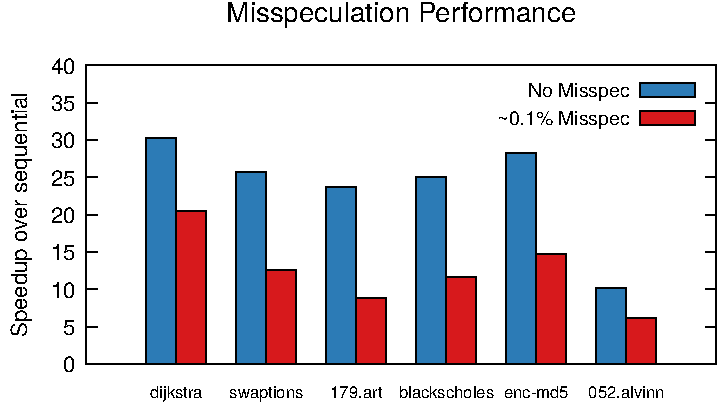
\includegraphics[width=\columnwidth]{figures/misspec-crop}
  \caption{Impact of misspeculation on benchmarks requiring speculation}
  \label{fig:misspec}
\end{figure}
Figure~\ref{fig:misspec} shows how misspeculation affects the
performance of the six of the eight speculative benchmarks with a misspeculation rate of
0.1\%.
Since none of the benchmarks exhibit misspeculation on the
given input sets, we artificially inject misspeculation at the end of
every 1000 iterations to observe the performance degradation.
Note that we do not evaluate the impact of misspeculation on \texttt{covariance}
or \texttt{correlation} as the only place misspeculation can occur is
during a heap check. Manually inspecting the source code reveals that this
will never fail.
% Note that misspeculation with \name is extremely unlikely, as
% static analysis can disprove many speculative assumptions and for many of
% the benchmarks, misspeculation is only possible during a heap check.
The inputs for \texttt{179.art} were not large enough to have
enough iterations for misspeculation at this rate, so we perform a
weighted average of non-misspeculating and misspeculating runs to achieve
an average corresponding to the respective rate.
These results demonstrate that \name performs well with only high
confidence speculation and requires tight integration with static analysis
to avoid heavy-weight speculation whenever possible.

% As the iteration within a checkpoint that misspeculation
% occurs can affect the recovery cost, we inject these misspeculations in the
% middle of a checkpoint chunk (\textbf{XXX} find better wording) to have a more
% realistic simulation, assuming that programs can misspeculate at any iteration with a
% uniform distribution.

% \subsection{Power Consumption}

% Power and energy stats here

